\section{Ablation Study}
\label{sec:ablation}
We ablate the two components of iPerturb, the context-specific GRN (evidence layers, cell-line tier, further databases, propagation kernels) and the learnable Hill propagation (transfer function, certified variant, loss), and the preprocessing. All differences are paired over unique held-out targets with 95\% bootstrap intervals (Table~\ref{tab:paired}).

\subsection{Evidence layers and controls}
\label{sec:ablation_layers}
Figure~\ref{fig:ablation}b summarises the layers of the GRN and the controls of Section~\ref{sec:results_pred}: STRING alone, the curated tier plus STRING, a degree-preserving rewired version, a graph learned from the training data, and the real graph with own-target entries zeroed. Only the real association evidence changes $\rho_c$ relative to no graph; the curated tier adds nothing beyond STRING, and controls with the same capacity and tuning grid gain nothing.

\subsection{Evidence tiers and multi-hop propagation}
\label{sec:ablation_tiers}
\begin{table}[t]
\centering
\caption{\textbf{Each evidence tier as a propagation graph, and multi-hop read-outs.} Unique-target mean $\rho_c$ over three target-held-out folds; the response of a held-out target is the propagated, normalised response of training targets over the graph, with the restart probability (or the number of hops) chosen on validation targets.}
\label{tab:tiers}
\footnotesize
\begin{tabular}{lcc}
\toprule
Graph (random walk with restart, $\alpha$ selected) & K562 $\rho_c$ & RPE1 $\rho_c$\\\midrule
Linear low-rank (B2) & 0.145 & 0.170\\
L1 curated (CollecTRI/OmniPath/TRRUST) & 0.131 & 0.162\\
L1 + SIGNOR & 0.146 & 0.175\\
L3 STRING & 0.298 & 0.313\\
L3 CORUM complexes & 0.263 & 0.278\\
L3 BioGRID physical & 0.241 & 0.264\\
L4 COXPRESdb & 0.173 & 0.208\\
L4 GTEx co-expression & 0.170 & 0.195\\
L2 ChIP-Atlas (cell line) & 0.130 & --\\
L1+L3, one hop (neighbour mean) & 0.282 & 0.301\\
L1+L3, random walk with restart (multi-hop) & 0.291 & 0.316\\
L1+L3, truncated 2--3 hops & 0.299 & 0.321\\
All tiers, propagated separately and integrated & 0.319 & 0.333\\
\bottomrule
\end{tabular}
\end{table}
We replaced the smoothing head by propagation of the observed training responses over each tier alone (Table~\ref{tab:tiers}) in the manner of network propagation~\cite{cowen2017network}. Association evidence of protein-level tiers carries the signal: STRING alone reaches $\rho_c=$ \datanum{g12_k562_prop_L3__rwr} (K562) and \datanum{g12_rpe1_prop_L3__rwr} (RPE1), CORUM complexes and BioGRID interactions are weaker but informative, whereas the curated regulatory tier (L1) and co-expression tiers (L4) stay near the linear baseline (\datanum{g12_k562_B2_linear} and \datanum{g12_rpe1_B2_linear}). Adding signed SIGNOR edges to L1 changes $\rho_c$ by \datanum{g12d_k562_signor_l1} (K562) and \datanum{g12d_rpe1_signor_l1} (RPE1). CORUM and BioGRID are worse than STRING (\datanum{g12d_k562_corum_l3} and \datanum{g12d_k562_biogrid_l3} in K562), and GTEx co-expression does not improve on COXPRESdb. Reading the same L1+L3 graph beyond the first hop helps: random walks with restart improve on the one-hop neighbour mean by \datanum{g12d_k562_rwr_one} (K562) and \datanum{g12d_rpe1_rwr_one} (RPE1), and truncated two- to three-step walks by \datanum{g12d_k562_trunc_one} and \datanum{g12d_rpe1_trunc_one}. Finally, propagating each tier separately and combining the read-outs with non-negative weights fitted on validation targets gives a further \datanum{g12d_k562_int_rwr} (K562) and \datanum{g12d_rpe1_int_rwr} (RPE1) over L1+L3 with random walks, and \datanum{g12d_k562_int_b2} and \datanum{g12d_rpe1_int_b2} over the linear baseline. The weights concentrate on the protein-association tiers (K562: STRING \datanum{g12w_k562_L3}, CORUM \datanum{g12w_k562_corum}, BioGRID \datanum{g12w_k562_biogrid}, COXPRESdb \datanum{g12w_k562_L4}, GTEx co-expression \datanum{g12w_k562_gtex_coex}, curated L1 \datanum{g12w_k562_L1}; RPE1: STRING \datanum{g12w_rpe1_L3}, CORUM \datanum{g12w_rpe1_corum}), so multi-hop propagation adds measurable accuracy, while the curated regulatory tier contributes explanation rather than prediction. The ChIP-Atlas cell-line tier (L2) does not improve over the linear baseline either (Table~\ref{tab:tiers}).

\subsection{Cell-line-specific tier}
\label{sec:ablation_context}
\datanumif{g7_d_k_hep}{\emph{Does the cell-line-specific tier carry cell-line-specific predictive signal?} We tested this in K562, the only line with a non-empty tier, with the smoothing head of Section~\ref{sec:results_pred} and a criterion registered before the run: the K562 tier must beat both foreign-line tiers. It does not. Adding the K562 GeneHancer tier to the L1+L3 graph changes the centred correlation by \datanum{g7_d_k_base} relative to the base graph, by \datanum{g7_d_k_hep} relative to adding the HepG2 tier and by \datanum{g7_d_k_jur} relative to the Jurkat tier; the enlarged graph is better than its degree-preserving rewired version, which also scrambles L1+L3, by \datanum{g7_d_k_rew}. The cell-line-specific tier therefore differs strongly between lines but adds no measurable predictive gain over generic association evidence in this setting.}

\subsection{Hill versus linear propagation}
\label{sec:ablation_hill}
Following the pre-registered gate, we trained the shared-Hill model and a linear model with the same graph, decoder and budget as a residual on the linear baseline for the reachable targets (\datanum{k562_g2_reach_n} K562 and \datanum{rpe1_g2_reach_n} RPE1 unique targets over three folds). All differences in the centred correlation are below 0.002 in either direction. The Hill form relative to the linear form is \datanum{k562_g2_h2_b3} in K562 and \datanum{rpe1_g2_h2_b3} in RPE1 (marginally positive in RPE1), relative to the linear baseline without graph \datanum{k562_g2_h2_b2} and \datanum{rpe1_g2_h2_b2}, and the real graph relative to a rewired graph is \datanum{k562_g2_h2_rew} and \datanum{rpe1_g2_h2_rew}; the pre-registered criterion (an advantage over both the linear form and the no-graph baseline, and over the rewired graph) was not met. An oracle readout with its scale fitted on the test targets themselves added nothing, so the limit is the information in the signed core rather than the optimiser. The conclusion is unchanged for a certified, anti-vanishing variant (log-odds state so that large responses are not squashed, a leaky Hill transfer that keeps a gradient where the curve is flat, a contraction guaranteed for every parameter value, Appendix~\ref{app:convergence}) trained with a correlation-based loss that does not shrink with the size of the response: relative to no graph, the Hill form changes $\rho_c$ on reachable targets by \datanum{g10d_k562_gn2_hill4_mse} (MSE) and \datanum{g10d_k562_gn2_hill4_corr} (correlation loss) in K562 and by \datanum{g10d_rpe1_gn2_hill4_mse} and \datanum{g10d_rpe1_gn2_hill4_corr} in RPE1 (Table~\ref{tab:certhill}); every interval includes zero. The Hill-form operator is therefore a faithful and efficient implementation of the regulatory model, not a source of additional predictive accuracy on this data.

\begin{figure}[t]
\centering
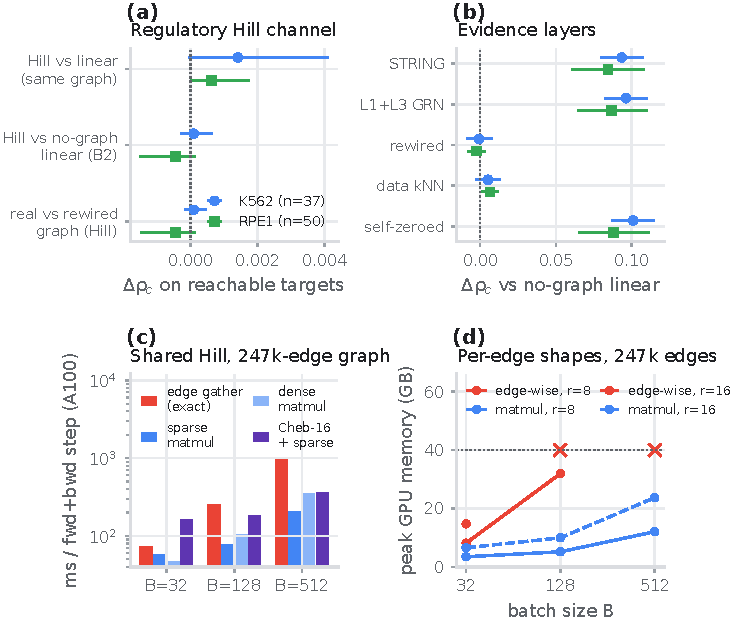
\includegraphics[width=\linewidth]{figures/fig4_ablation_efficiency.pdf}
\caption{\textbf{Ablations and efficiency.}
\textbf{(a)}~Hill-form versus linear propagation on the curated signed core, reachable test targets only (differences in $\rho_c$; \datanum{k562_g2_reach_n} K562 and \datanum{rpe1_g2_reach_n} RPE1 unique targets).
\textbf{(b)}~Change in $\rho_c$ relative to the no-graph linear model for evidence layers and controls (STRING only; L1+L3; rewired; graph learned from training data; L1+L3 with own-target entries zeroed).
\textbf{(c)}~Time per forward and backward step for the regulator-shared Hill operator on the 247k-edge association graph (A100).
\textbf{(d)}~Peak memory for edge-specific Chebyshev shapes (crosses: out of memory on 40\,GB).}
\label{fig:ablation}
\end{figure}

\subsection{Preprocessing}
\label{sec:ablation_prep}
Weighting training perturbations by cell number or by response precision did not help consistently (K562 \datanum{prep_k562_wn} and \datanum{prep_k562_wp} in $\rho_c$; RPE1 \datanum{prep_rpe1_wn} and \datanum{prep_rpe1_wp}), so the headline models are unweighted.
